\begin{figure}[t]
\centering
%% GATE: if the TikZ box exceeds the column width LaTeX does NOT WARN with an overfull hbox -- the box
%% silently spills over the neighboring column. We measure it and stop the build.
%% Measured (2026-09-11): box 210.7pt, \columnwidth 241.1pt.
\sbox0{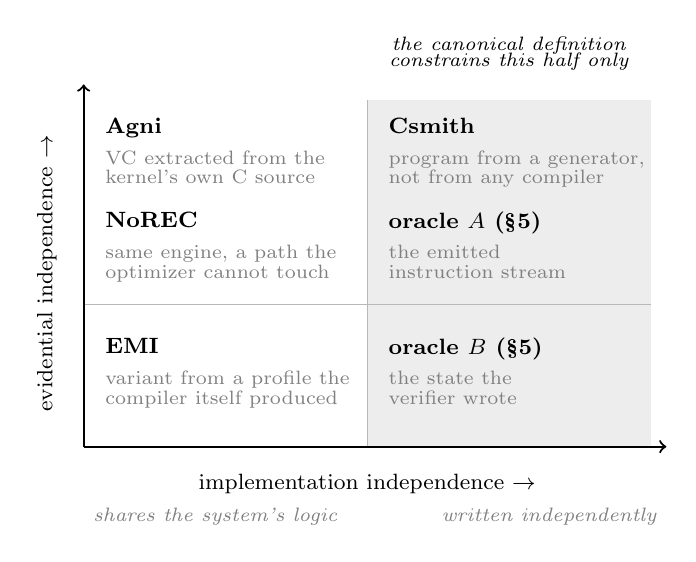
\begin{tikzpicture}[x=1mm,y=1mm,font=\footnotesize]
  \definecolor{gridgrey}{gray}{0.72}
  \definecolor{bandgrey}{gray}{0.93}
  %% Layout (B feedback): a column-filling width (76mm), a height cut in half
  %% (44mm), a font one size larger. Because the top half carries two entries
  %% (Agni, NoREC) it is taller than the bottom; the middle line is semantic, not a ratio.
  \fill[bandgrey] (36,0) rectangle (72,44);
  \draw[gridgrey] (0,18) -- (72,18);
  \draw[gridgrey] (36,0) -- (36,44);
  \draw[->,thick] (0,0) -- (74,0);
  \draw[->,thick] (0,0) -- (0,46);

  \node[anchor=north] at (36,-2.2) {implementation independence $\rightarrow$};
  \node[rotate=90,anchor=south] at (-2.2,22) {evidential independence $\rightarrow$};
  \node[anchor=north west,gray,font=\scriptsize\itshape] at (0,-6.5) {shares the system's logic};
  \node[anchor=north east,gray,font=\scriptsize\itshape] at (74,-6.5) {written independently};

  %% each entry is two nodes: a bold name + a gray two-line description
  \node[anchor=north west] at (1.5,43) {\textbf{Agni}};
  \node[anchor=north west,align=left,font=\scriptsize,text=gray] at (1.5,38.8) {VC extracted from the\\[-1pt]kernel's own C source};
  \node[anchor=north west] at (1.5,31) {\textbf{NoREC}};
  \node[anchor=north west,align=left,font=\scriptsize,text=gray] at (1.5,26.8) {same engine, a path the\\[-1pt]optimizer cannot touch};
  \node[anchor=north west] at (37.5,43) {\textbf{Csmith}};
  \node[anchor=north west,align=left,font=\scriptsize,text=gray] at (37.5,38.8) {program from a generator,\\[-1pt]not from any compiler};
  \node[anchor=north west] at (37.5,31) {\textbf{oracle $A$ (\S5)}};
  \node[anchor=north west,align=left,font=\scriptsize,text=gray] at (37.5,26.8) {the emitted\\[-1pt]instruction stream};
  \node[anchor=north west] at (1.5,15) {\textbf{EMI}};
  \node[anchor=north west,align=left,font=\scriptsize,text=gray] at (1.5,10.8) {variant from a profile the\\[-1pt]compiler itself produced};
  \node[anchor=north west] at (37.5,15) {\textbf{oracle $B$ (\S5)}};
  \node[anchor=north west,align=left,font=\scriptsize,text=gray] at (37.5,10.8) {the state the\\[-1pt]verifier wrote};
  \node[anchor=south,align=center,font=\scriptsize\itshape] at (54,46.5)
    {the canonical definition\\[-2pt]constrains this half only};
\end{tikzpicture}}%
\ifdim\wd0>\columnwidth
  \typeout{FIGWIDTH-ERROR box=\the\wd0 column=\the\columnwidth}%
\fi
\usebox0
\caption{The two axes, with the techniques of Section~7 placed on both. Height is
what an oracle reads: low means it reads what the system produced, high means it reads
something upstream of that. The shaded
half is what a pseudo-oracle is defined to be~\cite{barr2015oracle}: the condition
$f_1 \neq f_2$ fixes a horizontal position and says nothing about height. Agni and
oracle $B$ are mirror images---one encodes the component's own logic but reads its
source, upstream of every value it computes; the other is written independently but
reads what the component produced. Csmith occupies the corner it never claims: its
independence argument is made on the horizontal axis, while what protects it is its
height.}
\label{fig:axes}
\end{figure}
